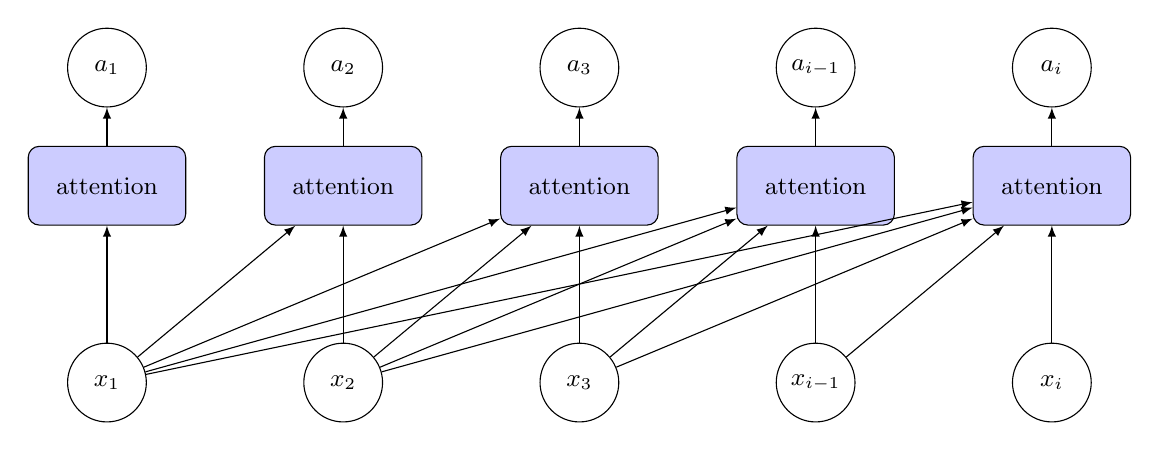
\begin{tikzpicture}[
    attention/.style={draw, fill=blue!20, rounded corners, font=\small, text centered, minimum width=2cm, minimum height=1cm},
    input/.style={draw, circle, minimum size=1cm, text centered, font=\small},
    output/.style={draw, circle, minimum size=1cm, text centered, font=\small},
    arrow/.style={->, >=latex}
]

% Inputs (x1 to x5)
\node[input] (x1) at (1, -1) {$\bm{x}_1$};
\node[input] (x2) at (4, -1) {$\bm{x}_2$};
\node[input] (x3) at (7, -1) {$\bm{x}_3$};
\node[input] (x4) at (10, -1) {$\bm{x}_{i-1}$};
\node[input] (x5) at (13, -1) {$\bm{x}_i$};

% Attention Blocks
\node[attention] (att1) at (1, 1.5) {attention};
\node[attention] (att2) at (4, 1.5) {attention};
\node[attention] (att3) at (7, 1.5) {attention};
\node[attention] (att4) at (10, 1.5) {attention};
\node[attention] (att5) at (13, 1.5) {attention};

% Outputs (a1 to a5)
\node[output] (a1) at (1, 3) {$\bm{a}_1$};
\node[output] (a2) at (4, 3) {$\bm{a}_2$};
\node[output] (a3) at (7, 3) {$\bm{a}_3$};
\node[output] (a4) at (10, 3) {$\bm{a}_{i-1}$};
\node[output] (a5) at (13, 3) {$\bm{a}_i$};

% Arrows from inputs to attention blocks
\draw[arrow] (x1) -- (att1);
\draw[arrow] (x2) -- (att2);
\draw[arrow] (x3) -- (att3);
\draw[arrow] (x4) -- (att4);
\draw[arrow] (x5) -- (att5);

% Arrows from attention blocks to outputs
\draw[arrow] (att1) -- (a1);
\draw[arrow] (att2) -- (a2);
\draw[arrow] (att3) -- (a3);
\draw[arrow] (att4) -- (a4);
\draw[arrow] (att5) -- (a5);

% Connections between inputs
\draw[arrow] (x1) -- (att2);
\draw[arrow] (x1) -- (att3);
\draw[arrow] (x1) -- (att4);
\draw[arrow] (x1) -- (att5);

\draw[arrow] (x2) -- (att3);
\draw[arrow] (x2) -- (att4);
\draw[arrow] (x2) -- (att5);

\draw[arrow] (x3) -- (att4);
\draw[arrow] (x3) -- (att5);

\draw[arrow] (x4) -- (att5);

\end{tikzpicture}
